\label{sec:BDT}
Boosted Decision Trees (BDTs) have a long history in high energy physics from enabling the first observation of single top production at the Tevatron~\cite{Abazov_2009} to helping in the discovery of the Higgs boson at the LHC~\cite{Aad_2012, Chatrchyan_2012}. A decision tree functions by making a series of cuts (or decisions) that maximize the separation between signal and background events in a single dimension. Each cut produces a branch in the tree containing independent populations. The depth of the tree sets the number of decisions a tree will make, and a well-designed tree will have end-nodes that efficiently separate and properly identify the constituent classes. Any series of cuts for identifying events will inevitably misclassify some events, and there are many strategies for improving the results. A boosted decision tree attempts to improve the classification by creating a new set of data from the improperly classified events and training a new decision tree on these inputs. Each step of re-training with misclassified events is called a \textit{boost}, and the total prediction for an event is the weighted sum of predictions from the orignal tree and the boosted trees where each sequential boost recieves a smaller weight in the sum.

The BDT trained for dihiggs detection was built using the xgboost package~\cite{xgboost}. The top seventeen reconstructed and event-level variables ranked by KS separability (discussed in Section~\ref{sec:eventReco}) were used in training. The hyperparameters describing the boosted decision tree were optimized for maximum $S/\sqrt{B}$. The optimal hyperparamters were found to be as follows: multiplicative boost factor of 0.1, maximum tree depth of 9, gamma (minimum loss reduction needed for further partition) of 1.1, and an L2 regularization term of 8.28.

\begin{figure}[!h]
\begin{center}
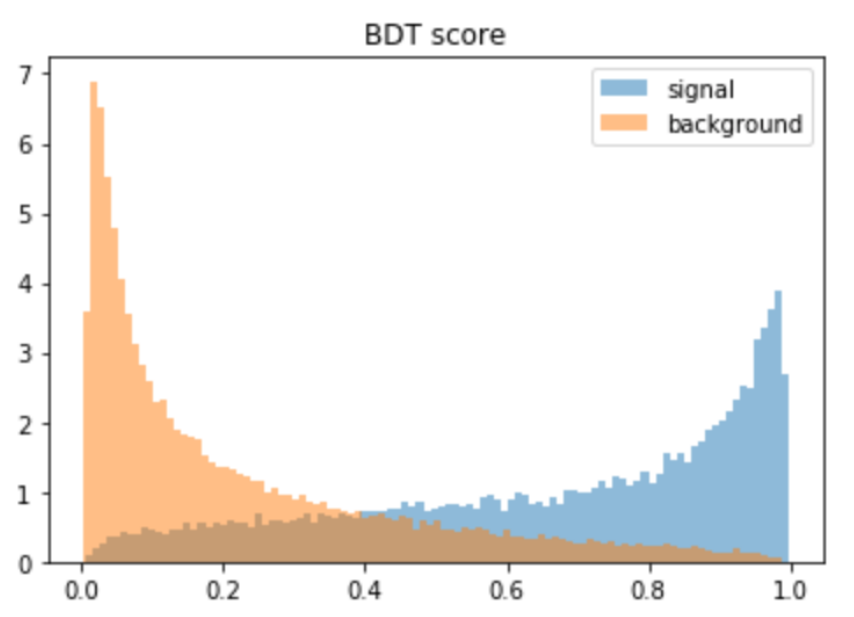
\includegraphics[width=3in]{BDT/bdt_pred}
\caption{Signal predictions of the trained BDT for signal and background samples independent from the training sets.}
\label{fig:bdt_pred}
\end{center}
\end{figure}

The predictions from the optimized BDT are shown in Figure~\ref{fig:bdt_pred}. A maximum significance of 1.84$\pm$0.09 was obtained, yielding 986 signal events and 2.8$\cdot 10^5$ background events. 
